%
%   Prof. Dr. Julian Reichwald
%   auf Basis einer Vorlage von Prof. Dr. Jörg Baumgart
%   DHBW Mannheim
%
%
%	ACHTUNG: Für das Erstellen des Literaturverzeichnisses wird das modernere Paket biblatex
%			 in Kombination mit biber verwendet -- nicht mehr das ältere BibTex!
% 			 Bitte stellen Sie ggf. Ihre TeX-Umgebung
% 			 entsprechend ein (z.B. TeXStudio: Einstellungen --> Erzeugen --> Standard Bibliographieprogramm: biber)
%

\documentclass[
	12pt,
	BCOR=5mm,
	DIV=12,
	headinclude=on,
	footinclude=off,
	parskip=half,
	bibliography=totoc,
	listof=entryprefix,
	toc=listof,
	pointlessnumbers,
	plainfootsepline,
	headings=optiontohead]{scrreprt}


%	Konfigurationsdatei einziehen
% !TEX root =  master.tex

%		LANGUAGE SETTINGS AND FONT ENCODING 
%
\usepackage[ngerman]{babel} 	% German language
\usepackage[utf8]{inputenc}
\usepackage{eurosym} % Euro symbol 
\usepackage[german=quotes]{csquotes} 	% correct quotes using \enquote{}
\usepackage[T1]{fontenc}
\usepackage{amssymb} % Mathe-Package
\usepackage{pdfpages} % for appendix pdfs


%\usepackage[english]{babel}   % For english language
%\usepackage{csquotes} 	% Richtiges Setzen der Anführungszeichen mit \enquote{}

% 		HYPERREF
%
\usepackage[
hidelinks=true % keine roten Markierungen bei Links
]{hyperref}

% Zwei eigene Befehle zum Setzen von Autor und Titel. Ausserdem werden die PDF-Informationen richtig gesetzt.
\newcommand{\TitelDerArbeit}[1]{\def\DerTitelDerArbeit{#1}\hypersetup{pdftitle={#1}}}
\newcommand{\AutorDerArbeit}[1]{\def\DerAutorDerArbeit{#1}\hypersetup{pdfauthor={#1}}}
\newcommand{\Firma}[1]{\def\DerNameDerFirma{#1}}
\newcommand{\Kurs}[1]{\def\DieKursbezeichnung{#1}}

\newcommand{\DieFachrichtungDerAusbildung}[1]{\def\DieFachrichtungDerAusbildung{#1}\hypersetup{pdftitle={#1}}}
\newcommand{\DieBerufsausbildung}[1]{\def\DieBerufsausbildung{#1}\hypersetup{pdfauthor={#1}}}

% Correct superscripts 
\usepackage{fnpct}


%		CALCULATIONS
%
\usepackage{calc} % Used for extra space below footsepline



%		BIBLIOGRAPHY SETTINGS
%

% Uncomment the next three lines for author-year-style with footnotes (Chicago)
\usepackage[backend=biber, autocite=footnote, style=authoryear, dashed=false]{biblatex} 	%Use Author-Year-Cites with footnotes
\AdaptNoteOpt\footcite\multfootcite   %will add  separators if footcite is called multiple consecutive times 
\AdaptNoteOpt\autocite\multautocite % will add  separators if autocite is called multiple consecutive times

% Uncomment the next line for IEEE-style 
% \usepackage[backend=biber, autocite=inline, style=ieee]{biblatex} 	% Use IEEE-Style (e.g. [1])

% Uncomment the next line for alphabetic style 
% \usepackage[backend=biber, autocite=inline, style=alphabetic]{biblatex} 	% Use alphabetic style (e.g. [TGK12])

% Uncomment the next two lines vor Harvard-Style 
%\usepackage[backend=biber, style=apa]{biblatex} 	
%\DeclareLanguageMapping{german}{german-apa}


\DefineBibliographyStrings{ngerman}{  %Change u.a. to et al. (german only!)
	andothers = {{et\,al\adddot}},
}

%%% Uncomment the following lines to support hard URL breaks in bibliography 
%\apptocmd{\UrlBreaks}{\do\f\do\m}{}{}
%\setcounter{biburllcpenalty}{9000}% Kleinbuchstaben
%\setcounter{biburlucpenalty}{9000}% Großbuchstaben


\setlength{\bibparsep}{\parskip}		%add some space between biblatex entries in the bibliography
\addbibresource{bibliography.bib}	%Add file bibliography.bib as biblatex resource


%		FOOTNOTES 
%
% Count footnotes over chapters
\usepackage{chngcntr}
\counterwithout{footnote}{chapter}

%	ACRONYMS
%%%
%%% WICHTIG: Installieren Sie das neueste Acronyms-Paket!!!
%%%
\makeatletter
\usepackage[printonlyused]{acronym}
\@ifpackagelater{acronym}{2015/03/20}
{%
	\renewcommand*{\aclabelfont}[1]{\textbf{\textsf{\acsfont{#1}}}}
}%
{%
}%
\makeatother

%		LISTINGS
\usepackage{listings}	%Format Listings properly
\renewcommand{\lstlistingname}{Quelltext}
\renewcommand{\lstlistlistingname}{Quelltextverzeichnis}
\lstset{numbers=left,
	numberstyle=\tiny,
	captionpos=b,
	basicstyle=\ttfamily\small,
	commentstyle=\itshape,
	breaklines=true, 
	breakatwhitespace=true,
	showstringspaces=false,
	escapeinside={@@},
	keywordstyle=\bfseries,
	postbreak=\raisebox{0ex}[0ex][0ex]{\ensuremath{\hookrightarrow\space}}
}

%LISTING inline a tabular/table
\newcommand\tablstinline[2][]{\lstinline[#1]{#2}}

% LISTINGS: eigene Programmiersprache; bei morekeywords die zusätzlichen einfügen
\lstdefinelanguage{PLSQL}{
	language     = SQL,
	morekeywords = {over, partition}}

% ---- LISTING FOR YAML FILES ----
%\usepackage[dvipsnames]{xcolor}
%\usepackage{listings}
\usepackage{color}
\newcommand\YAMLcolonstyle{\color{red}\mdseries}
\newcommand\YAMLkeystyle{\color{black}\bfseries}
\newcommand\YAMLvaluestyle{\color{black}\mdseries}

\makeatletter

% here is a macro expanding to the name of the language
% (handy if you decide to change it further down the road)
\newcommand\language@yaml{yaml}

\expandafter\expandafter\expandafter\lstdefinelanguage
\expandafter{\language@yaml}
{
	keywords={true,false,null,y,n},
	keywordstyle=\color{darkgray}\bfseries,
	basicstyle=\YAMLkeystyle,                                 % assuming a key comes first
	sensitive=false,
	comment=[l]{\#},
	morecomment=[s]{/*}{*/},
	commentstyle=\color{purple}\ttfamily,
	stringstyle=\YAMLvaluestyle\ttfamily,
	moredelim=[l][\color{orange}]{\&},
	moredelim=[l][\color{magenta}]{*},
	moredelim=**[il][\YAMLcolonstyle{:}\YAMLvaluestyle]{:},   % switch to value style at :
	morestring=[b]',
	morestring=[b]",
	literate =    {---}{{\ProcessThreeDashes}}3
	{>}{{\textcolor{red}\textgreater}}1     
	{|}{{\textcolor{red}\textbar}}1 
	{\ -\ }{{\mdseries\ -\ }}3,
}

% switch to key style at EOL
\lst@AddToHook{EveryLine}{\ifx\lst@language\language@yaml\YAMLkeystyle\fi}
\makeatother

\newcommand\ProcessThreeDashes{\llap{\color{cyan}\mdseries-{-}-}}
% --------------------------

%		EXTRA PACKAGES
\usepackage{lipsum}    %Blindtext
\usepackage{graphicx} % use various graphics formats
\usepackage[german]{varioref} 	% nicer references \vref
\usepackage{caption}	%better Captions
\usepackage{booktabs} %nicer Tabs
\newcommand{\ra}[1]{\renewcommand{\arraystretch}{#1}}
\usepackage{longtable} %multipages booktabs
\usepackage{array}
%\newcolumntype{P}[1]{>{\raggedright\arraybackslash}p{#1}}


%		ALGORITHMS
\usepackage{algorithm} %float wrapper for algorithms.
\usepackage{algpseudocode}
\renewcommand{\listalgorithmname}{Algorithmenverzeichnis }
\floatname{algorithm}{Algorithmus}


%		FONT SELECTION: Entweder Latin Modern oder Times / Helvetica
\usepackage{lmodern} %Latin modern font
%\usepackage{mathptmx}  %Helvetica / Times New Roman fonts (2 lines)
%\usepackage[scaled=.92]{helvet} %Helvetica / Times New Roman fonts (2 lines)

%		PAGE HEADER / FOOTER
%	    Warning: There are some redefinitions throughout the master.tex-file!  DON'T CHANGE THESE REDEFINITIONS!
%\RequirePackage[automark,headsepline,footsepline]{scrpage2}
\RequirePackage[automark,headsepline,footsepline]{scrlayer-scrpage}
\pagestyle{scrheadings}
\renewcommand*{\pnumfont}{\upshape\sffamily}
\renewcommand*{\headfont}{\upshape\sffamily}
\renewcommand*{\footfont}{\upshape\sffamily}
\renewcommand{\chaptermarkformat}{}
\RedeclareSectionCommand[beforeskip=0pt]{chapter}
\clearscrheadfoot


\ifoot[\rule{0pt}{\ht\strutbox+\dp\strutbox}DHBW Mannheim]{\rule{0pt}{\ht\strutbox+\dp\strutbox}DHBW Mannheim}
\ofoot[\rule{0pt}{\ht\strutbox+\dp\strutbox}\pagemark]{\rule{0pt}{\ht\strutbox+\dp\strutbox}\pagemark}

\ohead{\headmark}


\begin{document}

%TODO: Bitte passen!
%% BITTE GEBEN SIE HIER DEN TITEL UND DIE AUTORIN / DEN AUTOR DER ARBEIT AN!
%% DIESE INFORMATIONEN _MÜSSEN_ GESETZT SEIN, UM TITELBLATT, ABSTRACT UND
%% EIGENSTÄNDIGKEITSERKLÄRUNG AUTOMATISCH ANZUPASSEN!

\TitelDerArbeit{Ausbildung der Ausbilder: Unterweisung eines Auszubildenden}
\AutorDerArbeit{Yves Torsten Staudenmaier}
\Firma{SV Informatik GmbH}
\Kurs{WWI17SEC}
\DieFachrichtungDerAusbildung{Daten- und Prozessanalyse}
\DieBerufsausbildung{Berufsausbildung zur Fachinformatikerin (m/w/d)}

%---------------------------------------------------------------------------

\begin{titlepage}
\begin{minipage}{\textwidth}
		\vspace{-2cm}
		\noindent 
\includegraphics[scale=0.25]{img/ihk.eps} \hfill   
\includegraphics[scale=0.79]{img/logo.jpg}
\end{minipage}
\vspace{1em}
\sffamily
\begin{center}
	\textsf{\large{}Duale Hochschule Baden-W\"urttemberg\\[1.5mm] Mannheim}\\[2em]
	\textsf{\textbf{\Large{}ADA-Unterweisung }}\\[3mm]
	\textsf{\textbf{\DerTitelDerArbeit}} \\[1.5cm]
	\textsf{\textbf{\Large{}Studiengang Wirtschaftsinformatik}\\[3mm] \textsf{Studienrichtung Software Engineering}}
	
	\vspace{3em}
	%\textsf{\Large{Sperrvermerk}}
\vfill

\begin{minipage}{\textwidth}

\begin{tabbing}
	Wissenschaftlicher Betreuer: \hspace{0.85cm}\=\kill
	Verfasser/in: \> \DerAutorDerArbeit \\[1.5mm]
	Matrikelnummer: \> 7146590 \\[1.5mm]
%	Firma: \> \DerNameDerFirma  \\[1.5mm]
%	Abteilung: \> IE2 -- Deployment \\[1.5mm]
	Kurs: \> \DieKursbezeichnung \\[1.5mm]
	Studiengangsleiter: \> Prof. Dr.-Ing. habil. Dennis Pfisterer \\[1.5mm]
%	Wissenschaftlicher Betreuer: \> Marius Ebel \\
%	\> info@mariusebel.net \\
%	\> +49 176 / 473 45452 \\[1.5mm]
%	Firmenbetreuer: \> Thomas Teske \\
%	\> thomas.teske@sv-informatik.de \\
%	\> +49 621 / 454 44096 \\[1.5mm]
%	Bearbeitungszeitraum: \> 17.02.---08.05.2020
\end{tabbing}
\end{minipage}

\end{center}

\end{titlepage}

\pagenumbering{Roman} % Römische Seitennummerierung
\normalfont

%--------------------------------
% Verzeichnisse - nicht benötige Verzeichnisse bitte auskommentieren / löschen.
%--------------------------------

%   Sperrvermerk
%\chapter*{Sperrvermerk}
Der Inhalt dieser Arbeit darf weder als Ganzes noch in Auszügen Personen au"serhalb des Prüfungsprozesses und des Evaluationsverfahrens zugänglich gemacht werden, sofern keine anders lautende Genehmigung der Ausbildungsstätte vorliegt. Die Bachelorarbeit enthält unternehmensinterne Architektur- und Prozessmodellierung und deren Dokumentation. Es ist zum Zeitpunkt der Anmeldung nicht sicher, ob interne Schnittstellen in der Anwendungslandschaft offen gelegt werden.


%\vspace{3cm}
%\noindent\rule{5cm}{.4pt}\hfill\rule{5cm}{.4pt}\par
%\noindent Ort, Datum \hfill Unternehmensvertreter
%\cleardoublepage

\vspace{3cm}
\begingroup
\begin{table}[h!]
	\setlength\tabcolsep{0pt}
	\begin{tabular}{p{6.5cm}p{8.5cm}}
		Mannheim, 05.05.2020 &  \\
		& \\
		& Nadja Haumbach, Ausbildungsverantwortliche \\
	\end{tabular}
\end{table}


% Lesehinweis
\chapter*{Lesehinweise}
Die folgenden Hinweise sollen das Lesen dieser Projektarbeit erleichtern und spezielle Formatierung definieren:

\begin{itemize}
	\item Im Sinne der Gleichberechtigung wird in dieser Arbeit entweder die Form \textit{\enquote{die Entwickler*in}} oder die grammatikalisch korrekte Form \textit{\enquote{die/der Entwickler/-in}} verwendet werden. Bei der Kurzform mit der Sternnotation wird auf Grund der Lesbarkeit der weibliche Artikel benutzt.
	\item Produkt- oder Eigennamen werden in \textsc{Kapitälchen} gesetzt, wie beispielsweise \textsc{Node.js}.
	\item Hochgestellte Ziffern weisen auf Fußnoten am Seitenende hin.
	
\end{itemize}
 

%	Kurzfassung
%\chapter*{Kurzfassung}
\addcontentsline{toc}{chapter}{Abstract}
\begingroup
\begin{table}[h!]
\setlength\tabcolsep{0pt}
\begin{tabular}{p{3.7cm}p{11.7cm}}
Titel & \DerTitelDerArbeit \\
Verfasser/in: & \DerAutorDerArbeit \\
Kurs: & \DieKursbezeichnung \\
Ausbildungsstätte: & \DerNameDerFirma\\
\end{tabular}
\end{table}
\endgroup

%Überlege, ob ich den Header brauche mit den ganzen Infos?
%Hier können Sie die Kurzfassung der Arbeit schreiben. 



%	Inhaltsverzeichnis
\tableofcontents

%	Abbildungsverzeichnis
\listoffigures 

%	Tabellenverzeichnis
\listoftables

%	Listingsverzeichnis
%\lstlistoflistings
 

% 	Algorithmenverzeichnis
%\listofalgorithms

% 	Abkürzungsverzeichnis (siehe Datei acronyms.tex!)
\clearpage
\chapter*{Abkürzungsverzeichnis}	
\addcontentsline{toc}{chapter}{Abkürzungsverzeichnis}


\begin{acronym}[RDBMS]
	\acro{AWL}{Anwendungslandschaft}
	\acro{DHBW}{Dualen Hochschule Baden-Württemberg}
	\acro{BaFin}{Bundesanstalt für Finanzdienstleistungsaufsicht}
	\acro{BSI}{Bundesamt für Sicherheit in der Informationstechnik}
	\acro{VAIT}{Versicherungsaufsichtliche Anforderungen an die IT}
	\acro{IE2}{IE2 -- Deployment}
	\acro{IE}{IE -- Entwicklungs- und Betriebsunterstützung}
	\acro{CAB}{\enquote{Change Advisory Board}}
	\acro{ITIL}{Information Technology Infrastructure Library}
	\acro{SV}{SV SparkassenVersicherung}
	\acro{SVI}{SV Informatik GmbH}
	\acro{SVS}{SV Sachsen}
	\acro{i.d.R.}{in der Regel}

\end{acronym}

\ohead{Acronyms} % Neue Header-Definition

%--------------------------------
% Start des Textteils der Arbeit
%--------------------------------
\clearpage
\ihead{\chaptername~\thechapter} % Neue Header-Definition (inner header)
\ohead{\headmark} % Neue Header-Definition (outer header)
\pagenumbering{arabic}  % Arabische Seitenzahlen

%	Anleitungs-Datei anleitung.tex einziehen. Auf diese Weise sollten Sie versuchen, für jedes einzelne
% Kapitel eine eigene Datei anzulegen und mittels input-Kommando einzuziehen.
%\input{anleitung}

%-----------------
% Kapitel einbinden
%-----------------


% reset memory of all acronyms, so \ac will print out full name of acronym!
\acresetall 

\chapter{Einleitung}

\chapter{Rahmenbedingungen}

\section{Auszubildende}
Die Auszubildende \Azubi begann ihre Ausbildung im September 2018 -- somit befindet sie sich im 22. Monat ihrer Ausbildung. Annalena hat eine sehr gute mittlere Reife und ist 19 Jahre alt. Sie hat im Rahmen der Ausbildung einige Abteilungen durchlaufen und kennt dadurch die Wertschöpfungskette der \ac{SVI}. Viel wichtiger ist jedoch, dass sie durch den Einsatz in verschiedenen Abteilungen viele Mitarbeitende kennt und im Unternehmen positiv bekannt ist. Die persönliche Eignung hat den Betrieb bei der Einstellung von Annalena überzeugt: ihre ständige Neugierde, ihre Fähigkeit sich zu fokussieren, ihr Wunsch etwas zu lernen und ihr Verlangen nach sinnhafter Arbeit führten sie mit guten bis sehr guten Leistungen durch die Ausbildung. Bevor sie in die Abteilung \enquote{Geschäftsanalytik} kam, war sie in diversen Abteilungen, die sich mit Datenaufbereitung, -validierung und -vorbereitung beschäftigt haben. Damit hatte sie ein Teil der Fertigkeiten, Kenntnisse und Fähigkeiten aus §4 Absatz 5 Nummer 3 \ac{FIAusbV} erfolgreich erworben. Dieses Vorwissen bildet die Grundlage für diese Unterweisen.

\section{Ausbildungsbetrieb}
Der Ausbildungsbetrieb \ac{SVI} ist eine Tochtergesellschaft der \ac{SV}, die die IT-Dienstleitungen für ihren Mutterkonzern sowie die \ac{SVS} übernimmt. Die Gesellschaften gehören dem S-Finanzbund an. Bei der \ac{SVI} handelt es sich um ein mittelständiges Unternehmen mit dem Firmensitz Mannheim und ungefähr 450 Mitarbeitenden\autocite[vgl.][]{sv_informatik_gmbg_uber_2020} an fünf Standorten in Deutschland. Die Standorte Mannheim, Dresden, Kassel, Stuttgart und Wiesbaden sind im Geschäftsgebiet der \ac{SV} und \ac{SVS} verteilt. \enquote{Unseren Kunden bieten wir ein \enquote{Rund-um-Sorglos-Paket}[sic!]: Von der Beratung, über Konzepte bis hin zur produktiven Anwendung. Und das alles auf Basis moderner Infrastrukturen und Plattformen.}\autocite{sv_informatik_gmbg_uber_2020}
\par
Die Ausbildung der Fachinformatiker*innen erfolgt an allen Standorten. Ziel der Ausbildung ist es, die Handlungskompetenz der Auszubildenden zu fördern und sie bestmöglich auf den Einsatz an den verschiedenen Standorten vorzubereiten. Deswegen sind die Ausbildungsstationen auf alle Standorte verteilt.

\section{Ausbilder/-in}
Der Ausbilder Max Müller hat ein erfolgreich abgeschlossenes Studium in Wirtschaftsinformatik. Er arbeitet seit dem 01.~Juni 2015 bei der \ac{SVI} und bekleidet aktuell die Stelle eines \enquote{Senior Developer} im Bereich maschinellem Lernen. Herr Müller ist fachlich gemäß §30\,BBiG geeignet, da er ein Hochschulstudium absolviert hat und fünf Jahre in diesem Beruf praktisch tätig ist. Des Weiteren ist Herr Müller persönlich gemäß §29\,BBiG geeignet, da er Jugendliche beschäftigen darf und nicht gegen das \ac{BBiG} oder auf Grund des \ac{BBiG} erlassenen Vorschriften oder Bestimmungen wiederholt oder schwer verstoßen hat. Somit erfüllt er die Voraussetzung der Eignung eines Ausbilders gemäß §28\,BBiG. Außerdem hat er im Rahmen seines Studiums die Veranstaltung zum Erlangen des Ada-Scheins erfolgreich besucht. Die Aufgabe des Ausbilders ist es, einen guten Umgang mit den Auszubildenden in der Rolle des Coachs, Mentors, Erziehers und des Vorbilds zu pflegen. Er ist bedacht ein gutes Betriebsklima aufrecht zu halten, um eine positive Lernatmosphäre für seine Auszubildenden zu begünstigen.

\section{Lernort}
Da die Verfügbarkeit eines eigenen Büros nicht gegeben ist, wird für die Unterweisung ein Besprechungsraum reserviert. Zwar ist das Großraumbüro kein geeigneter Ort, um eine Unterweisung durchzuführen, da keine ruhige und lernfördernde Atmosphäre entstehen kann -- allerdings wird der großzügige Besprechungsraum so präsentiert, sodass keine ungewollten Ablenkungsmöglichkeiten für den Auszubildenden und den Ausbilder entstehen können. Das Telefon im Raum wird deaktiviert und der Raum jeweils 20 Minuten vor und nach der Unterweisung blockiert, damit kein Zeitdruck während dieser Zeit entsteht. Auch ist der Ausbilder 25 Minuten vor dem Eintreffen des Auszubildenden im Besprechungsraum, um alles vorzubereiten. Der Raum ist dem Auszubildenden bekannt und mit großen Fenstern in Blickrichtung des Innenhof des Gebäudes versehen, sodass viel Tageslicht eindringen kann. Durch die großen Fenster kann für eine angenehme Lüftung und Temperatur gesorgt werden. Falls es doch zu warm werden sollte, verfügt das Gebäude über eine Klimaanlage. Die Möblierung ist angemessen und in freundlichen Farben gehalten. Der Raum ist gegenüber Lärm abgeschottet. 

\section{Unterweisungszeitpunkt und -dauer}
Der Ausbilder ist sich der Tatsache des menschlichen Biorhythmus und dessen unterschiedliche Ausprägung bei verschiedenen Menschen bewusst. Er weiß aus früheren Gesprächen mit der Auszubildenden Annalena Schmidt, dass sie gern sehr früh morgens anfängt zu arbeiten und in den frühen Morgenstunden am leistungsfähigsten ist. Auf Grund dieses Gesprächs wird die Unterweisung für morgens um 9 Uhr angesetzt. Auch der Ausbilder ist, wie Frau Schmidt, meist früh am Arbeitsplatz. Die Unterweisung dauert maximal 20 Minuten. Dieser Zeitraum teilt sich in folgende Bestandteile auf: die Begrüßung, ein kurzer Small-Talk, die Unterweisung, die Erfolgskontrolle, die Zeitreserve und die Verabschiedung.

\section{Unterweisungsmethode}
In dieser Unterweisung wird die fragend-entwickelnde Methodik des Lehrgesprächs verwendet. Dabei wird darauf geachtet Fragen, konstruktive Einwände und sonstige Beteiligung des Auszubildenden nicht zu unterbinden. Somit wird auch der affektive Lernbereich erreicht. 

\section{Lehr- und Arbeitsmittel}
Als Lehr- und Arbeitsmittel werden folgende Materialien bereitgestellt: 
%TODO: Nochmal anpassen!
\begin{itemize}
	\item Laptop mit installierter Software, die für die Unterweisung benötigt wird,
	\item Schreibutensilien, wie Papier und Stifte, 
	\item ein kleines Informationsplakat, dass das Vorgehen des Algorithmus zeigt;
	\item Zusammenfassung des Gelernten,
	\item Übungsaufgaben und 
	\item Zugang zu den Simulationsdateien.
\end{itemize}



\chapter{Lernziele, -bereiche und -kontrolle}

\section{Lernziele}
Grundsätzlich ist das Lernen eine Verhaltensänderung, die 

\begin{itemize}
	\item durch Versuch, Irrtum und zufälligen Erfolg;
	\item durch Nachahmung oder 
	\item durch Einsicht
\end{itemize}

bewirkt wird. Belohnung eines gezeigten Verhaltens wirken als positiver Verstärker. Kurz definiert ist Lernen \enquote{die Veränderung einer Verhaltensweise durch Erfahrung}.
\par
Im Kern der Unterweisung geht es um das Lernen. Deswegen ist den Lernzielen besondere Aufmerksamkeit zu schenken. Lernziele sollen möglichst genau angeben welche Verhaltensweisen in welchem Maße und unter welchen Bedingungen geändert werden sollen. 

\subsection{Richtlernziel}
Die Richtlernziele sind der \ac{FIAusbV} zu entnehmen: Gemäß §3 Absatz 1 FIAusbV\autocite[][§3 I FIAusbV]{bundesminister_fur_wirtschaft_und_energie_verordnung_2020} sind mindestens die im Ausbildungsrahmenplan genannten Fertigkeiten, Kenntnisse und Fähigkeiten Gegenstand der Ausbildung. Diese Ziele sind als \enquote{Teil des Berufsbildes} im Ausbildungsrahmenplan beschrieben. 
\par
Die vorliegende Unterweisung thematisiert das Richtlernziel des Abschnitts D \enquote{Nutzen der Daten zur Optimierung von Arbeits- und Geschäftsprozessen sowie zur Optimierung digitaler Geschäftsmodelle}\autocite[vgl.][§4 V Nr.\,3 FIAusbV]{bundesminister_fur_wirtschaft_und_energie_verordnung_2020}. Dieses Richtlernziel richtet sich an die Fachrichtung \enquote{Daten- und Prozessanalyse} und ist deswegen den berufsprofilgebenden Fertigkeiten, Kenntnissen und Fähigkeiten dieser Fachrichtung zugeordnet.

\subsection{Groblernziel}
Das Groblernziel wird durch die Beschreibung der zu vermittelnden Fertigkeiten, Kenntnisse und Fähigkeiten des Ausbildungsrahmenplan illustriert. Dieses Ziel konkretisiert welche Fertigkeiten, Kenntnisse und Fähigkeiten der Auszubildende nach dem Abschluss der Ausbildung beherrschen soll. Jedoch ist das Groblernziel zu unspezifisch formuliert, um es direkt zur Erfolgskontrolle zu nutzen. 
\par
Ziel der vorliegenden Unterweisung ist es, einen Beitrag zur Vermittlung der Groblernziele Nr.\,4f \enquote{mathematische Vorhersagemodelle anwenden} und Nr.\,4g \enquote{Werkzeuge zur Mustererkennung und Modellgenerierung nutzen} zu leisten. Diese Ziele sind dem Auszubildenden ab dem 19. bis zum 36. Monat zu vermitteln. Da sich die beiden Ziele ergänzen, sollen beide in die Entwicklung des Feinlernziels der Unterweisung einfließen. 
 
\subsection{Feinlernziel}
Das Feinlernziel soll operationalisiert sein: Die genaue Zielsetzung beschreibt eine exakte Erläuterung des Lernziels mit allen Einzelheiten, die gut überprüfbar sein müssen. Daraus folgt, dass das Lernziel dann operationalisiert ist, wenn überprüfbare Verhaltensweisen festgelegt sind, anhand derer der Auszubildende geprüft werden kann. 

\begin{table}[h!]
	\centering
	
	\begin{tabular}{@{}cp{8.0cm}l@{}}
		\toprule
		\textbf{Nummer} & \textbf{Feinlernziel} & \textbf{Stufe} \\ \midrule
		1 & Die allgemeine Vorgehensweise nennen, um ein Cluster zu erzeugen & Reproduzieren\\
		2 & Die Idee des Algorithmus \enquote{k-means} nennen & Reproduzieren \\
		3 & Einzelne Schritte des Algorithmus nennen, fehlende erkennen und auswerten & Reorganisation \\
		4 & Die benötigten Werkzeuge zur Mustererkennung und Modellgenerierung nennen und fehlende erkennen & Reorganisation \\ 
		5 & Gute und schlechte Cluster erkennen & Reorganisation \\
		6 & Selbstständig neue Daten mittels des Algorithmus gruppieren & Transfer \\ 
		7 & Daten gruppieren, die nicht mittels des erlernten Algorithmus einteilbar sind & Kreativität\\ 

		\bottomrule
	\end{tabular}

	\caption{Feinlernziele der Unterweisung}
	\label{tab:lernziele}
\end{table}

Das Feinlernziel sieben ist ein langfristiges Ziel und beschränkt sich nicht auf diese einzelne Unterweisung, sondern soll mittels sich wiederholenden Unterweisungen erreicht werden.

\section{Lernbereiche}
Hier werden die einzelnen Lernbereiche angesprochen, jedoch ist der psychomotorische Bereich nicht genannt, da diese Unterweisung diesen Lernbereich nicht ansprechen wird.

\subsection{Kognitiver Bereich}
Der kognitive Lernbereich umfasst das berufliche Wissen sowie geistige Operationen zu erlernen. Dabei ist der Fokus auf das Wissen beschränkt. 
\par
Die Auszubildende Sabrina Dengel lernt ein Cluster-Verfahren kennen, dass gewisse Kenntnisse erfordert. Sie lernt die allgemeine Vorgehensweise und einen Algorithmus, um ein Cluster zu finden. Außer lernt sie die Programmiersprache \textsc{Python} als Werkzeug zur Mustererkennung.

\subsection{Affektiver Bereich}
Dieser Bereich beschreibt die Fähigkeit des Auszubildenden bestimmte Einstellungen, Werthaltungen und Anschauungen zu erlernen. Es geht hier um die gefühlsmäßigen Bereiche.
\par
Die Auszubildende lernt die Wichtigkeit der richtigen Anwendung des Verfahrens kennen. Auch lernt sie die Ergebnisse zu interpretieren und damit eine gewisse Werthaltung gegenüber eines Ergebnisses zu besitzen.

%\subsection{Psychomotorischer Bereich}

\section{Erfolgskontrolle}\label{kap3:erfolg}
Es werden im Anschluss der Unterweisung Kontrollfragen gestellt, die zeigen, ob das Gelernte verstanden wurde. Auch bekommt die Auszubildende Übungsaufgaben und eine kurze Zusammenfassung ausgehändigt, um die Unterweisung selbstständig nochmals nachvollziehen zu können. Die Übungsaufgaben soll Sabrina innerhalb von zwei Wochen während ihrer Arbeitszeit erledigen und dem Ausbilder vorlegen. Die Aufgaben sind so gewählt, dass die Auszubildende weder über- noch unterfordert wird.
\par
Um das Gelernte zu festigen und den Erfolg zu kontrollieren, wird Sabrina im Anschluss an die Unterweisung folgende Informationen erhalten: Ihr wird eine Ansprechpartnerin genannt bei der sie sich melden soll, um das Gelernte auf andere Daten in Zusammenarbeit mit der Ansprechpartnerin weiter zu üben. Schließlich wird Sabrina die nächsten vier Wochen die Ansprechpartnerin begleiten und nach ihren Fähigkeiten, Kenntnissen und Fertigkeiten unterstützen. Der Ausbilder informiert die Ansprechpartnerin über das Vorhaben und kontrolliert auch, dass dieses die Auszubildende weder über- noch unterfordert. 



\chapter{Motivation}

\paragraph{intrinsische Motivation}
Die intrinsische Motivation ist das innere, aus sich selbst entstehende Inzentiv eines Menschen. Bestimmte Tätigkeiten werden durch die intrinsisch motivierte Person ihres selbst Willens ausgeübt, da sie Spaß machen, sinnvoll bzw. herausfordernd oder interessant sind. Wichtig ist, dass diese Art der Motivation nicht durch Belohnungen entsteht oder konditioniert wird. Der Ausbilder kann nur durch die Funktion des Vorbildes diese Motivation ansprechen, in dem sie/er für eine Tätigkeit brennt bzw. diese total spannend und toll findet. Dies kann dann auf den Auszubildenden überspringen. 
\par
Der Ausbilder brennt für das Thema sehr und hofft dieses Gefühl durch sein Verhalten auf die Auszubildende Sabrina Dengel zu übertragen. Er hofft, dass sie nach der Unterweisung genau so viel Interesse verspürt. Wenn der Ausbilder nur einen kleinen Teil seiner Begeisterung auf seine Auszubildende übertragen durch die Funktion des Vorbilds, ist das Motivieren von der Auszubildenden geglückt. 

\paragraph{extrinsische Motivation}
\hyphenation{Ent-wick-lungs-ge-mäß-heit}
% ---------------------------------------------
\chapter{Pädagogische bzw. didaktische Prinzipien}
In diesem Kapitel werden die einzelnen didaktischen Prinzipien kurz erläutert und auf die vorliegende Unterweisung übertragen. Es ist naheliegend, dass alle genannten pädagogischen Prinzipien in die Unterweisung einfließen, um einen bestmöglichen Erfolg zu unterstützen. Die allgemeinen Grundsätze für die didaktischen Überlegungen gelten unbeschränkt: 

\begin{itemize}
	\item vom Leichtem zum Schweren,
	\item vom Einfachen zum Zusammengesetzten, 
	\item vom Nahen zum Entfernten, 
	\item vom Allgemeinen zum Speziellen und 
	\item vom Konkreten zum Abstrakten.
	
\end{itemize}

\section{Prinzip der Anschaulichkeit}
Anschauung bezeichnet das bewusste, eindringliche, absichtliche und allseitige Erfassen eines Gegenstandes mit möglichst allen Sinnen. Ein solches allseitiges Aufnehmen eines Gegenstandes ist die Grundlage für den weiteren geistigen Prozess einer Unterweisung.\autocite[vgl.][S.\,161ff.]{schroder_lernen_2010} Allgemein gilt der Grundsatz: Anschauen $\Rightarrow$ Denken $\Rightarrow$ Anwenden.
\par
Um dieses Prinzip umzusetzen, bringt der/die Ausbilder/-in ein Informationsplakat mit dem zu vermittelnden Algorithmus mit. Auch eine anschaulich Simulation des Ablaufs des Algorithmus wird mitgebracht. Die Auszubildende kann damit anschaulich diesen nachvollziehen. Sie bekommt die Unterlagen nach der Unterweisung zur Verfügung gestellt, um eine Hilfestellung für die Aufgaben der Erfolgskontrolle zu haben.

\section{Prinzip der Aktivität}
Bei diesem Prinzip kann die/der Ausbilder/-in sich den Tätigkeitsdrang der Jugendlich zunutze machen: Aktive und selbstständige Mitarbeitende sind für jeden Betrieb unerlässlich. Auch kann die demokratische Gesellschaft ohne aktive Mitarbeitende und kritisch denkende Staatsbürger/-innen nicht bestehen.
\par
Durch das fragend-entwickelnde Lehrgespräch ist \Azubi dazu angehalten kritisch und aktiv mitzudenken, damit ist sie aktiviert und eingebunden. Auch soll sie selbstständig im Lehrgespräch das mitgebrachte Schaubild ergänzen. Dabei zieht sie selbst Rückschlüsse durch das Wissen, das sie sich in der Vergangenheit angeeignet hat. Schließlich versucht \Azubi das Wissen zu übertragen. 

\section{Prinzip der Praxisnähe}
Die Auszubildenden, die geeignet für den Ausbildungsberuf sind, sind daran interessiert sinnvolle Arbeit zu leisten, d.\,h., sie möchten etwas lernen, das in der beruflichen Praxis verwertbar ist. Übertragen bedeutet das, es ist darauf zu achten nur aktuelle und praxisnahe Fertigkeiten, Kenntnisse und Fähigkeiten zu vermitteln. 
\par
Die Exploration bzw. die automatische Wissensgenerierung mittels Computersystem ist heutzutage nicht mehr wegzudenken. Die Unternehmen besitzen immer mehr Daten ihrer Kunden, ihres Unternehmens und ihrer Konkurrenten.\autocite[vgl.][]{noauthor_hochschule_nodate}\autocite[vgl.][]{noauthor_volkswagen_nodate} Diese Datenflut muss mit mathematischen Methoden unter Zuhilfenahme von Computersystem aufbereitet werden, da Mitarbeitende ohne Hilfe die große Menge von Daten nicht bewältigen können. Maschinelles Lernen beschreibt dieses Vorgehen. Die \ac{SVI} entwickelt Systeme im Bereich des maschinellen Lernens für ihre Kundin \ac{SV}. Damit ist das Thema der Unterweisung direkt aus dem operationalen Geschäftsfeld des Ausbildungsbetriebes. 

\section{Prinzip der Entwicklungsgemäßheit}
Dieses Prinzip beschreibt, dass die körperliche und/oder geistliche Überforderung des Auszubildenden unbedingt zu vermeiden ist. Weiterhin ist zu beachten, dass die Art und Weise wie ein/-e Jugendliche/-r denkt oder fühlt sich stark von der eines Erwachsenen unterscheiden kann. Übertragen bedeutet das: Die/der Ausbilder/-in hat auf den individuellen Entwicklungsstandes des Auszubildenden einzugehen. 
\par
In der vorliegenden Unterweisung wird darauf geachtet, dass die Sprache und die Intensität der Wissensvermittlung an die Auszubildende angepasst wird. Der Ausbilder achtet drauf, dass Sabrina Dengel an ihrem Kompetenz- und Interessenniveau abgeholt wird. Damit wird einer Über- oder Unterforderung entgegengewirkt. Wichtig hierbei ist die Anpassung der Sprache und des Anspruches an den Auszubildenden.

\section{Prinzip der Erfolgssicherung}
Dieses Prinzip gehört zu den obersten Leitsätzen einer jeden Unterweisung: Die/der Ausbilder/-in möchte, dass das vermittelte Wissen beim Auszubilden fest verankert wird, damit es im weiteren Verlauf der Ausbildung und im späteren Berufsalltag verwendet werden kann. 
\par
Die Erfolgssicherung wird ausführlich in Kapitel \vref{kap3:erfolg} beschrieben. Eine weitere Ausführung bedarf es aus der Sicht des Autors nicht.

\section{Prinzip der Verknüpfung}
Hier wird explizit die Wissensverknüpfung in den Mittelpunkt gestellt. Es sollen Anknüpfungspunkte für den Auszubildenden geschaffen werden, an denen sie/er sich festhalten kann, um das neu erlernte Wissen in Verknüpfung zum bereits Gelernten zu bringen. Die Anknüpfungspunkte können aus dem Betrieb oder dem Alltag kommen. Hier fließt das Prinzip der didaktischen Reduktion \enquote{vom Einfach zum Schweren und vom Bekannten zum Unbekannten} ein.
\par
Sabrina Dengel hat in vorhergehenden Abteilung einige Anknüpfungspunkte zum Thema der Unterweisung sammeln können. So hat sie auch in der Berufsschule eine Einführung in den Themenkomplex des maschinellen Lernens erhalten. In der vorliegenden Unterweisung wird Sabrina Dengel ein weiteres Verfahren der Clusteranalyse kennen lernen. 


\chapter{Handlungskompetenz}

\chapter{Planung der Unterweisung}
% Please add the following required packages to your document preamble:
% \usepackage{booktabs}
% \usepackage{multirow}
% \usepackage{longtable}
% Note: It may be necessary to compile the document several times to get a multi-page table to line up properly
\begin{longtable}[c]{@{}lp{3.5cm}p{4.5cm}p{4.0cm}@{}}
	\toprule
	\textbf{Phase}                        & \textbf{Lernschritt}                         & \textbf{Kernpunkt}                                                                                                                                        & \textbf{Begründung}                                               \\* \midrule
	\endfirsthead
	%
	\multicolumn{4}{c}%
	{{\bfseries Tabelle \thetable\ von vorheriger Seite fortgesetzt.}} \\
	\toprule
	\textbf{Phase}                        & \textbf{Lernschritt}                         & \textbf{Kernpunkt}                                                                                                                                        & \textbf{Begründung}                                               \\* \midrule
	\endhead
	%
	\multirow{4}{*}{\textit{Eröffnung}}   & Begrüßung                                    & Angenehme Lernatmospähre herstellen, Etwas Small-Talk (nicht zu persönlich)                                                                               & Abbau möglicher Hemmungen gegenüber dem Ausbilder                 \\* \cmidrule(l){2-4} 
	& Thema\&Ziel                                  & Kurze Erläuterung des Themas und Beschreibung des Lernziels; den Sinn der Unterweisung kurz umreisen bzgl. der Anwendung in der Abteilung                 & Transparenz, Überblick, Sinnhaftigkeit erkennen                   \\* \cmidrule(l){2-4} 
	& Motivation                                   & Azubi hat n. d. Unterweisung einen Wissensvorsprung (Anerkennung durch das Umfeld, extrin.); Ausbilder brennt für dieses Thema (Vorbildfunktion, intrin.) & Trägt zur Lernbereitschaft bei                                    \\* \cmidrule(l){2-4} 
	& Vorkenntnisse                                & Durch offene Fragen Vorkenntnisse finden (Was kannst du mir zum Thema Clusterverfahren erzählen?)                                                         & Anknüpfungspunkte finden                                          \\* \midrule
	\multirow{6}{*}{\textit{Erarbeitung}} & \multirow{2}{*}{Einstieg}     & Was ist ein Cluster? Was stellst du dir darunter vor?                                                                                                     & \multirow{6}{*}{offene Fragen}                                    \\* \cmidrule(lr){3-3}
	&                                              & Welche Eigenschaften könnten genutzt werden, um die Cluster zu bilden?                                                                                    &                                                                   \\* \cmidrule(lr){2-3}
	& \multirow{2}{*}{Erarbeitung} & Wie könnte der Algorithmus vorgehen, um die oben genannten Eigenschaft zur Einteilung zu nutzen?                                                          &                                                                   \\* \cmidrule(lr){3-3}
	&                                              & Welche Voraussetzungen müssen gegeben sein, damit der Algorithmus funktioniert?                                                                           &                                                                   \\* \cmidrule(lr){2-3}
	& \multirow{2}{*}{Abschluss}                   & Welche Anwendungsfälle könntest du dir vorstellen?                                                                                                        &                                                                   \\* \cmidrule(lr){3-3}
	&                                              & Welche Vorteile kannst du dir bei dem Algorithmus vorstellen? Welche Nachteile?                                                                           &                                                                   \\* \midrule
	\multirow{4}{*}{\textit{Schluss}}     & Erfolgskontrolle                             & Siehe dazu Kapitel XKAPX                                                                                                                                  & Überprüfung des Erlernten; Erkennung von möglichen Lücken         \\* \cmidrule(l){2-4} 
	& Ausblick                                     & Nächstes Thema: Weiteres Clustering-Verfahren (dbscan) + Vergleich der beiden Verfahren                                                                   & Überblick, Transperanz und Neugierde wecken                       \\* \cmidrule(l){2-4} 
	& Berichtsheft                                 & Hinweis auf die Pflicht diese Unterweisung einzutragen; Kontroll-Termin ankündigen                                                                        & Reflexion des Erlernten; Zulassungsvoraussetzung Abschlussprüfung \\* \cmidrule(l){2-4} 
	& Verabschiedung                               &                                                                                                                                                           & Positives Ende                                                    \\* \bottomrule
	\caption{Zeitlicher und fachlicher Unterweisungsplan}
	\label{tab:Unterweisungsplan}
\end{longtable}

%-----------------

\clearpage
\pagenumbering{Roman}
\setcounter{page}{7} %TODO: schauen, ob die "9" passt.

%	Literaturverzeichnis
\printbibliography[title=Literaturverzeichnis]
\cleardoublepage

% Der Anhang beginnt hier - jedes Kapitel wird alphabetisch aufgezählt. (Anhang A, B usw.)
\appendix
\ihead{\appendixname~\thechapter} % Neue Header-Definition

% appendix.tex einziehen
\addcontentsline{toc}{chapter}{Anhang} %sorgt für eintrag ins inhaltsverzeichnis
\chapter{Ausschnitt der zugrunde liegender Ausbildungsordnung}

	\begin{center}
		\fbox{\includegraphics[height=0.9\textheight, page=15]{reference/VO_Fachinformatiker_2020}}	
	\end{center}
	
	\newpage
	\begin{center}
		\fbox{\includegraphics[height=0.97\textheight, page=16]{reference/VO_Fachinformatiker_2020}}
	\end{center}



% Ehrenwörtliche Erklärung ewerkl.tex einziehen
% !TEX root =  master.tex

\clearpage
\chapter*{Ehrenwörtliche Erklärung}

% Wird die folgende Zeile auskommentiert, erscheint die ehrenwörtliche
% Erklärung im Inhaltsverzeichnis.
\addcontentsline{toc}{chapter}{Ehrenwörtliche Erklärung}

Ich versichere hiermit, dass ich die vorliegende Arbeit
 mit dem Thema: \textit{\DerTitelDerArbeit} selbstständig verfasst und keine anderen als die angegebenen Quellen und
Hilfsmittel benutzt habe. Ich versichere zudem,
dass die eingereichte elektronische Fassung mit der gedruckten Fassung übereinstimmt.

\vspace{3cm}
\noindent\rule{5cm}{.4pt}\hfill\rule{5cm}{.4pt}\par
Ort, Datum \hfill \DerAutorDerArbeit



\end{document}
